\startchapter{The Large Hadron Collider and the ATLAS Experiment}
\label{chapter:lhcatlas}

The \textbf{Large Hadron Collider (LHC)} is the world's largest and most energetic proton-proton collider. It is located within a 27 km circular ring beneath Switzerland and France, below towns, farmland, and part of the Jura mountains next to the \textbf{Conseil Européen pour Recherche Nucléaire (CERN)} in suburban Geneva. It began operation in 2008, and since then has collided over $10^{15}$ particles. The collider houses four major experiments: ALICE, ATLAS, CMS, and LHCb, along with several smaller projects. ALICE (A Large Ion Collider Experiment) studies heavy ion collisions, while LHCb (Large Hadron Collider beauty) specializes in studying the physics of the bottom quark. \textbf{ATLAS (A Toroidal LHC ApparatuS)} and CMS (Compact Muon Solenoid) are both general purpose experiments designed to study a wide range of interactions resulting from high-energy proton-proton collisions. This work uses data collected by the ATLAS experiment, and a description of the LHC accelerator and ATLAS detector follow in Sections \ref{section:lhc} and \ref{section:atlas}.

\section{The Large Hadron Collider}
\label{section:lhc}
Built between 1998 and 2008, the LHC \cite{LHCDesign} began colliding protons in 2010 at a center-of-mass energy of 7 TeV, and most recently from 2015 to 2018 collisions occured at 13 TeV. Successfully colliding particles at this energy is an immense technical challenge which is achieved by the many technologies of the LHC and its accelerator complex.

In order to reach a beam energy of 6.5 TeV, protons are slowly stepped up in energy through a chain of accelerators before reaching the LHC. They begin their journey as hydrogen molecules, which are ionized into bare protons before being accelerated to an energy of 50 MeV by the Linac2 linear accelerator. Following this, the Proton Synchrotron Booster (PSB) accelerates them to 1.4 GeV, passing them to the Proton Synchrotron (PS) and the Super Proton Synchrotron to be accelerated to 25 and then 450 GeV. Finally, beams are split into clockwise and counterclockwise directions and injected into the LHC where they are accelerated to their final 6.5 TeV energy. The CERN accelerator complex, including this injection system as well as surrounding experiments is shown in Figure \ref{fig:lhc_injector}.

\begin{figure}[h!]
    \centering
    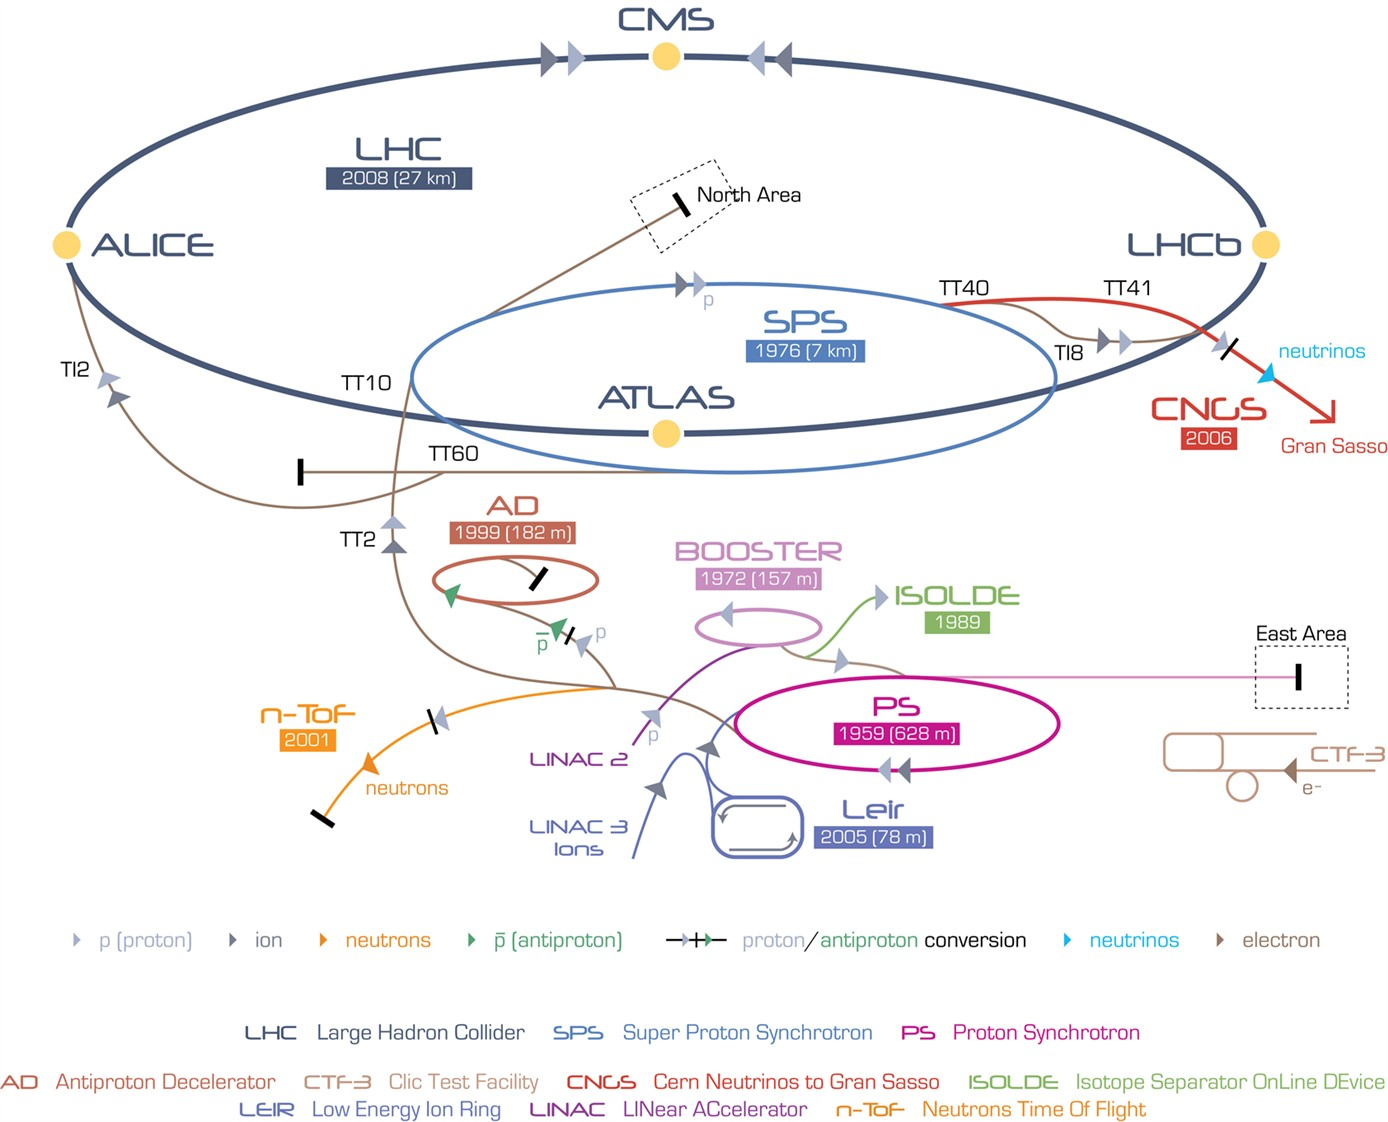
\includegraphics[width=0.8\textwidth]{Figures/2/cern_complex.png}
    \caption{Overview of the CERN accelerator complex, including the LHC injector system and the main surrounding experiments.}
    \label{fig:lhc_injector}
\end{figure}

The acceleration of the protons is achieved by radio-frequency cavities. These cavities contain a resonant electromagnetic field oscillating at 400 MHz, which is applied to particles passing through. The LHC contains 8 cavities per beam, with each providing a maximum of 2 MV of potential, so each proton can recieve up to 16 MeV of energy per lap. As a result it takes millons of laps over a period of around 20 minutes for a proton injected at 450 GeV to reach its collision energy of 6.5 TeV.  These RF cavities also help to keep each beam in bunches of $1.15 \times 10^{11}$ protons spaced at intervals of just 25 ns.

The crown jewels of LHC technology are its magnets. The LHC contains 1,232 superconducting NbTi dipole magnets kept at 1.9 K, each spanning 14.3 m and weighing 35 tonnes, with each creating an 8.3 Tesla magnetic field. This field lies perpendicular to the beam path, bending the beams along their desired route. The bending dipole magnets are complemented by 392 quadrupole magnets that focus the beams to a small aperture, and many higher-order multipole magnets which provide small beam corrections.

Together with the collisional energy of the accelerated particles, the other most important measure of a particle acceletator is the luminosity it achieves. \textbf{Luminosity ($\mathcal{L}$)} is used to determine the rate ($R$) at which a given interaction occurs using:
\begin{equation}
R = \mathcal{L}\sigma,
\end{equation}
where $\sigma$ is the cross-section of the desired interaction. As a result, when searching for rare processes, obtaining a high luminosity is crucial.

The integrated luminosity, $L$, gives the total number of interactions over a period of time, and is defined as:
\begin{equation}
L = \int \mathcal{L}\, dt.
\end{equation}
At the LHC, the luminosity is controlled by the number $n_b$ of bunches circulating , the frequency of revolution $f_r$, the numbers $N_{1,2}$ of particles in each colliding bunch, and the cross sectional area of the colliding beams. This results in the equation:
\begin{equation}
\mathcal{L}  = \frac{ f_rn_bN_1N_2 }{4\pi\sigma_x\sigma_y}R_{\phi},
\end{equation}
where $R_{\phi}$ is a geometrical loss factor caused by the beams crossing at an angle, and $\sigma_{x,y}$ are the horizontal and vertical widths of the beams (which, to a good approximation, have Gaussian cross-sectional profiles). The LHC currently has a nominal peak luminosity of $\mathcal{L} = 10^{34} cm^{-2}s^{-1}$.

\section{The ATLAS Experiment}
\label{section:atlas}

The ATLAS experiment \cite{ATLASDesign} uses the LHC in combination with the ATLAS detector to test a broad range of SM and BSM predictions. Together with the CMS experiment, its greatest achievement to date was the detection and discovery of the SM Higgs boson in 2012 \cite{HiggsDiscovery}.

\begin{figure}[H]
    \centering
    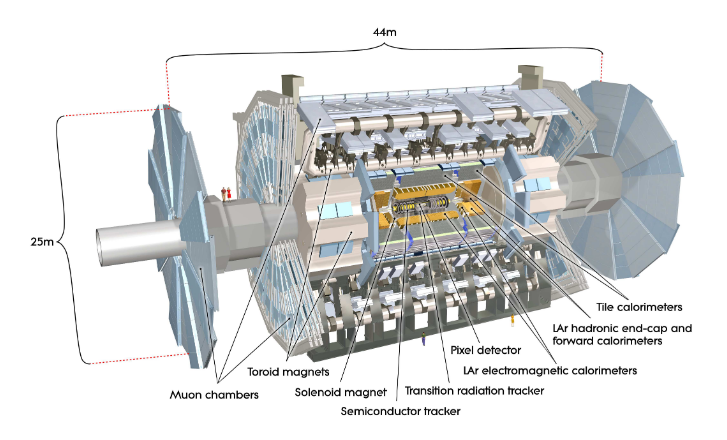
\includegraphics[width=0.8\textwidth]{Figures/2/ATLASDetector.png}
    \caption{A cut-out overview of the ATLAS detector and main components. Diagram from \cite{ATLASDesign}.}
    \label{fig:atlasdec}
\end{figure}

The ATLAS detector, an overview of which is shown in Figure \ref{fig:atlasdec}, is comprised of several layers of sub-detectors, which work in tandem to detect many diverse particles. From inner-most to outer-most the layers are:

\begin{itemize}
    \item the \textbf{inner detector}, which in turn contains the pixel detector, the semiconductor tracker, and the transition radiation tracker, and which has excellent angular resolution to track charged particles,
    \item the \textbf{electromagnetic calorimeters}, designed primarily to measure the energy and position of electrons and photons,
    \item the \textbf{hadronic calorimeters}, designed to measure the energy and position of hadrons,
    \item the \textbf{muon spectrometer}, to track and measure muons.
\end{itemize}

When combined with the electronics required to read out and trigger on measurements, the entire detector weighs over 7000 t and measures 44 m long by 25 m wide and high. Its barreled shape with end caps covers nearly the full solid angle. The following sections will describe the layout and operations of the ATLAS detector in more detail.

\subsection{Inner Tracking Detector}
The ATLAS inner detector tracks the direction and momentum of charged particles immediately after the particles leave the interaction point. A 2 T superconducting solenoid surrounds the inner detector, bending charged particles via the Lorentz force, allowing their momentum to be determined from the curvature of their path. Within the inner detector, there are three separate sub-detectors: the \textbf{Pixel Detector}, the \textbf{Semiconductor Tracker (SCT)}, and the \textbf{Transition Radiation Tracker (TRT)}. A cutout view of the detector is shown in Figure \ref{fig:atlasinner}.

\begin{figure}[H]
    \centering
    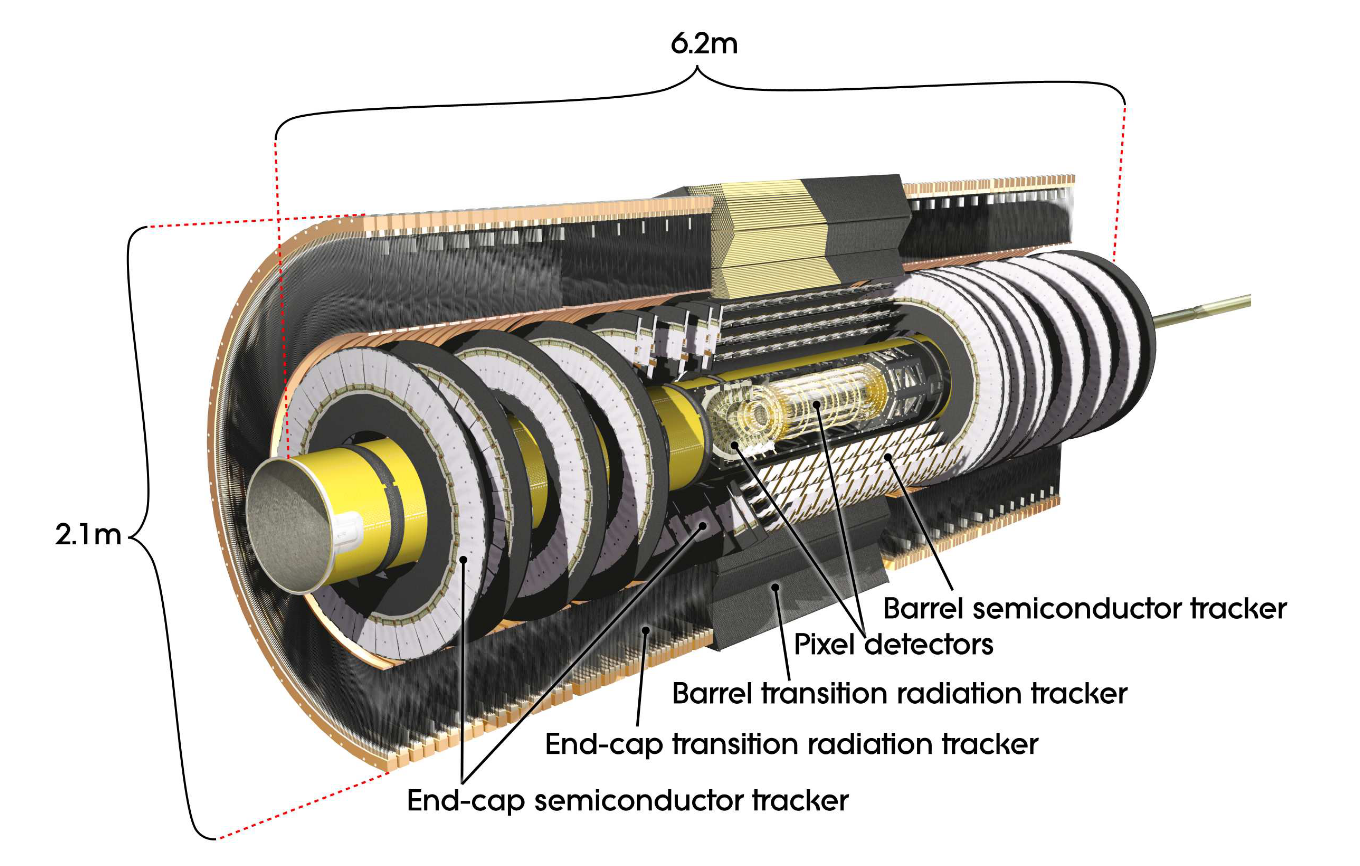
\includegraphics[width=0.8\textwidth]{Figures/2/InnerDetector.png}
    \caption{A cut-out view of the ATLAS inner detector. Diagram from \cite{ATLASDesign}.}
    \label{fig:atlasinner}
\end{figure}

The Pixel Detector consists of an array of 1744 pixel sensors, each containing 47232 silicon pixels, with most of these pixels each measuring 50x400 $\mu m^2$. They are arranged into three cyclindrical layers in the barrel and three disk-shaped layers on each end. The high granularity of these detectors ensures strong angular resolution, providing precise measurements of vertex location and track momentum. Notably, this detector must be very radiation-hard in order to maintain performace over the detector lifespan, as the pixel detector is the ATLAS subdetector that receives the highest radiation dose from the intense particle flux.

Though it would be desirable, it would not be feasible to extend the high-resolution pixel detector because of the high cost and signal readout volume. As a result, in the SCT the small rectangular pixels are extended into silicon strip detectors, which are laid in pairs at an angle of 40 mrad to each other to allow measurements in two dimensions. The SCT is made up of four concentric cylindrical layers in the barrel and two disk-shaped layers on each end-cap.

The TRT is the final component of the component of the inner detector.  It consists of approximately 300000 drift tubes, primarily filled with Xenon gas, with the wall of each tube kept at -1.5 kV relative to a central wire at ground. When particles pass through the tubes, the gas is ionized and the resulting electrons drift to the center and are collected on the central wire.  The electrical signal pulse is then amplified within electronics at the end of each wire. Additionally, the gaps between TRT straws are filled with polymer fibres (in the barrel) or foils (in the end caps). As a result, highly relativistic particles create transition radiation at the material interfaces, which aids with electron identification.

\subsection{Calorimeters}
The ATLAS calorimeter system measures the energies and positions of both charged and neutral particles after they leave the inner detector. In addition to measuring the energy of each particle, the calorimeters must contain enough material to stop the vast majority of particles (with the exception of muons and undetected neutrinos) from reaching the muon spectrometers. To acheive this, high-density passive layers interact with passing particles and cause them to decay into showers, dispersing their energy. These layers are interleaved with active layers that detect the decaying showers to measure particle energy.

\begin{figure}[H]
    \centering
    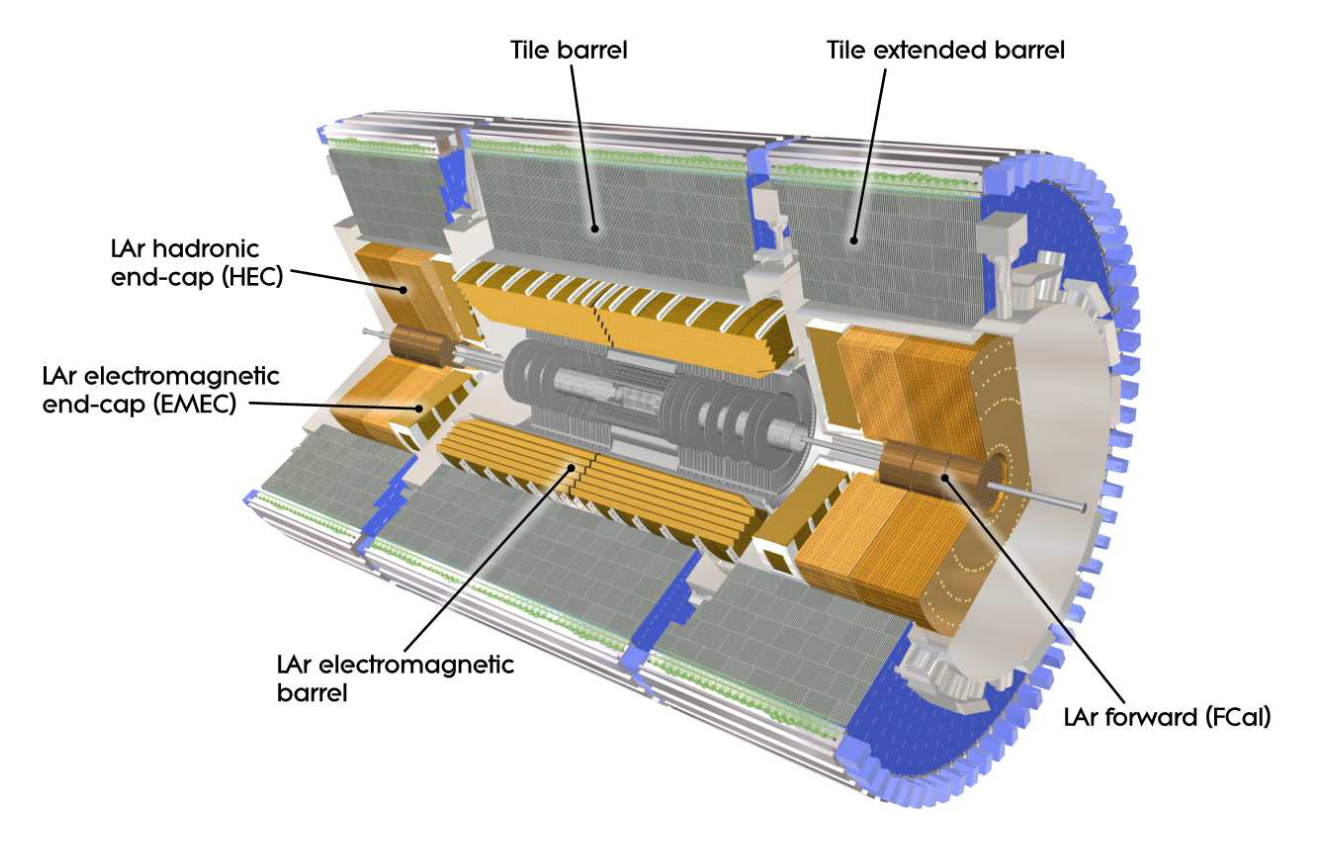
\includegraphics[width=0.8\textwidth]{Figures/2/Calo.png}
    \caption{A cut-out view of the ATLAS calorimeter system. Diagram from \cite{ATLASDesign}.}
    \label{fig:atlascalo}
\end{figure}

The ATLAS calorimeters can be categorized into electromagnetic (EM) calorimeters which measure the energy of electrons and photons, and hadronic calorimeters which primarily measure the energy of hadrons. ATLAS uses a combination of two different calorimeter technologies to form these detectors. In the end-cap and forward regions Liquid Argon (LAr) is used as the active layer in both the hadronic and EM calorimeters, while in the barrel region plastic scintillating tiles are employed in the hadronic calorimeter. Figure \ref{fig:atlascalo} depicts the layout of the ATLAS calorimeter system.

\subsubsection{Electromagnetic calorimeters}
The electromagnatic LAr calorimeter lies just outside the solenoid surrounding the inner detector. Layers of lead are used as the passive material. In the lead, electrons and photons interact with the closely spaced atoms, initiating a cascading shower of decays. The charged electrons in the shower pass through the active layers and ionize the LAr inside. The electrons and ions then drift across the 2 kV difference to opposite electrodes, where they are amplified into an electrical signal.

Like the inner detector, the LAr EM calorimeter can be divided into an \textbf{Electromagnetic Barrel (EMB)} calorimeter and two \textbf{Electromagnetic End-Cap (EMEC)} calorimeters. In the barrel region, the layers are placed together in a folded accordion-like geometry to create uniformity and allow easy electronic readout. An overview of this accordion-style layout is shown in Figure \ref{fig:accord}. The barrel and end-cap regions are 53 cm and 63 cm thick respectively, and cover a minimum of 22 and 24 radiation lengths ($X_0$), keeping shower leakage to a minimum.

\begin{figure}[H]
    \centering
    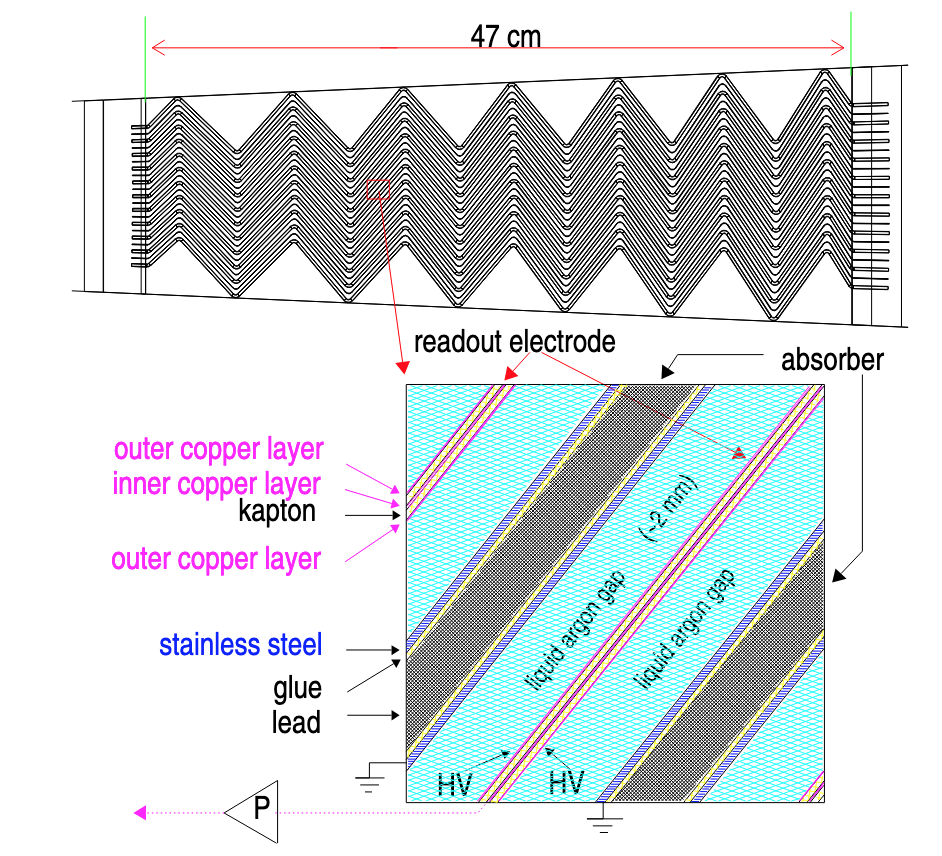
\includegraphics[width=0.6\textwidth]{Figures/2/accordion.png}
    \caption{A schematic demonstrating the components and accordion-like geometry of the ATLAS LAr EM calorimeter. Diagram from \cite{Accordion}.}
    \label{fig:accord}
\end{figure}

\subsubsection{Hadronic Calorimeters}
In the end cap regions, the \textbf{Hadronic End-Cap (HEC)} calorimeter shares a similar design to the EM LAr calorimeters, but with copper as the passive absorbing material between active layers. In the barrel region, the hadronic calorimetry is performed by the \textbf{Tile Calorimeter} with plastic scintillators as the active detectors. Particle showers passing through the plastic tiles produce scintillating light, which is directed to photomultipliers to be converted to an electrical signal. In the tile calorimeter, steel is the passive material laid between active layers. The depth of the combination of electromagnetic and hadronic calorimeters is important to prevent particles from punching through to the background-sensitive muon spectrometer. The total thickness, including supporting materials, is approximately 11 interaction lengths, which keeps punch-through below the levels of irreducible backgrounds in the muon spectrometer, and also ensures an accurate measurement of $E^{miss}_T$ as very little energy escapes measurement.

The final calorimeter in the ATLAS detector is the \textbf{Forward Calorimeter (FCal)}, located nearest the beam path. It has three layers of passive absorbing metals: an inner copper layer optimized for electromagnetic measurements and two outer tungsten layers to measure hadronic interactions. It too employs liquid argon as the active material, this time in a matrix of longitudinal channels parallel to the beam line.

\subsection{Muon Spectrometers}
After the calorimeters have stopped the vast majority of particles exiting the interaction point, muons and neutrinos remain undetected. The ATLAS experiment does not directly detect neutrinos, and instead reconstructs them from missing transverse momentum, however muons are measured by the muon spectrometer. A diagram of the muon system is shown in Figure \ref{fig:muon_system}. The centerpiece of this system is an arrangement of three air-core toroidal magnets, a barrel toroid and two end-cap toroids. Each toroid consists of eight coils in loops in a radially-symmetric pattern around the beam line. Together they form a 4 T magnetic field to bend muons.

\begin{figure}[H]
    \centering
    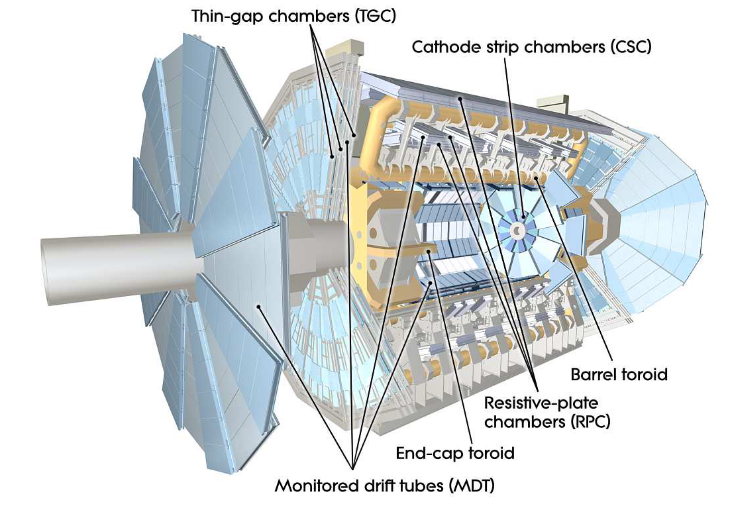
\includegraphics[width=0.8\textwidth]{Figures/2/muon_system.png}
    \caption{A cut-out view of the ATLAS muon spectrometer system. Diagram from \cite{ATLASDesign}.}
    \label{fig:muon_system}
\end{figure}

Four different detector types are used to measure the muons. \textbf{Monitored Drift Tubes (MDTs)} are pressurized gas drift tubes that collect ionized electrons to measure track coordinates in the bending direction of the magnetic field. They are supplemented by finer-grained and more radiation-hard \textbf{Cathode Strip Chambers (CSCs)} at $|\eta | > 2$. \textbf{Resistive Plate Chambers (RPCs)} and \textbf{Thin Gap Chambers (TGCs)} measure the muon track coordinares in the direction orthogonal to the magnetic bending direction, and are also used by the trigger system to provide bunch-crossing indentification and $p_T$ thresholds.

\subsection{Trigger and Data Acquisition}
The ATLAS detector can detect as many as 1.7 billion proton-proton collisions per second, but to save and process all of the information from each collision would require a prohibitive amount of readout electronics, computing power, and storage space. Instead, the trigger system quickly selects events based on key observables to slim down the data.  On the detector itself, the \textbf{Level-1 (L1) trigger} uses custom electronics within the detector, and works with reduced granularity information from the muon chambers and calorimeters to select potentially interesting events with high-$p_T$ objects or high $E^{miss}_T$. The detector readout systems can handle a maximum acceptance rate of 100 kHz from the L1 trigger. The \textbf{Level 2 (L2) trigger} is outside the detector and uses traditional computing resources. It takes regions of interest where the L1 trigger finds interesting objects and reconstructs them more fully to further reduce the event rate below 3.5 kHz. Together with the L2 trigger, the \textbf{event filter} forms the second half of the \textbf{High-Level Trigger (HLT)}. At this stage, events are fully reconstructed before being further filtered to a rate of approximately 200 Hz to be stored and analyzed offline.
